\chapter{Desenvolvimento do Projeto}
\label{chap:desenv}

As ferramentas escolhidas para o desenvolvimento do projeto foram a Unity3D para a criação da aplicação, ASP.NET Core para a REST API e React para o dashboard administrativo.
 
\section{Estrutura}
\label{sec:estrutura}

\begin{figure}[htb]
\caption{\label{fig:estrutura} Estrutura do projeto}
\begin{center}
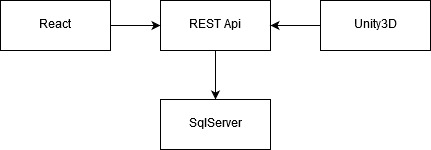
\includegraphics[scale=0.75]{Estrutura}
\end{center}
\legend{Fonte: própria} 
\end{figure}

A aplicações se comunicam com o servidor por meio do protocolo REST.

\section{REST API}
\label{sec:restapi}



\subsection{Visão Geral}
\label{subsec:visaogeral}

A API serve como centro do projeto. Ela guarda todas as questões, usuários, opções e os rankings. Ela decide também quais e quantas questões um jogador irá receber quando uma nova partida for requisitada. Os clientes e a API se comunicam através do protocolo REST, enviando e recebendo JSONs.

A API é implementado em C\# utilizando o ASP NET Core 2.2 e Entity Framework Core para acesso ao banco de dados. Seguindo o padrão MVC o projeto é dividido em 3 partes, os Controllers que representam a camada de Views, as Business que representam a camada de Controllers e os Repositories que representam a camada de Models.

\subsection{Usuários}
\label{subsec:usuários}

Os usuários são representados pela classe user. Cada usuário tem um Username único e uma lista de roles que determinam quais funcionalidades da API o usuário tem acesso. A senha do usuário é passada pelo algoritmo HMAC-SHA521 e somente o hash resultante e o salt utilizados são salvos no banco.

Um usuário pode ser tanto um jogador como um administrador, podendo ser ambos dependendo das Roles dadas ao usuário. 

A função da API para criação de usuários é a aberta, por tanto qualquer um pode se registrar, porém usuários criados assim só terão acesso às funções de jogador. Um administrador pode depois dar a um usuário acesso às funções de administração.

\subsection{Controle de Acesso}
\label{subsec:acesso}

Cada função da API restringe seu acesso dependendo das Roles que ela requer de um usuário acessado. Existem 2 Roles no sistema “admin” e “user” que dão acesso às funções de administração e às funções do jogo respectivamente.

Algumas funções não requerem um usuário logado, como a função de cadastro e login, e outras só requerem que o usuário esteja logado, sem se importar com quais Roles eles possuem.

\subsection{Questões}
\label{subsec:questoes}

Cada questão possui um enunciado, uma flag indicando se essa questão está ativa e deveria ser enviada aos jogadores e um número aleatório utilizando para escolha das questões para um jogador. Opcionalmente uma questão pode ter uma imagem e varios Temas e Categorias. 

Cada questão deve ter exatamente 4 respostas com somente uma sendo marcada como correta para poder ser marcada como ativa. 

\subsubsection{Respostas}
\label{subsubsec:respostas}

Cada resposta tem um texto, uma flag indicando se essa resposta é correta e opcionalmente uma imagem. 

Uma resposta está sempre ligada a uma única questão e somente uma resposta ligada a cada questão pode ser marcada como correta. 


\subsubsection{Escolhendo Questões}
\label{subsubsec:escolhendo}

Quando um jogador começa uma nova partida a API escolhe quais questões para enviar para o jogador. A escolha é feita aleatoriamente entre as questões ativas que o jogador ainda não tenha respondido. 

Primeiramente as questões são filtradas para conterem somente questões ativas que o jogador não tenha respondido ainda. Depois um número aleatório é gerado e é feito um “ou exclusivo” entre este número e o número aleatório de cada questão e as questões são ordenadas de acordo com os números resultantes. Por fim a quantidade necessária de questões é pega a partir do começo da lista.

Caso depois do processo não existam questões suficientes para uma partida, a lista de questões que o jogador já respondeu é apagada e o processo é repetido excluindo as questões que já tenham sido escolhidas anteriormente e o número de questões faltando são escolhidas. Se mesmo assim não houverem questões suficientes a partida começa com questões faltando.

\subsection{Partidas}
\label{subsec:partidas}

Uma partida começa com o jogador requisitando o começo de uma nova partida para a API e recebendo as questões a serem respondidas. 

Uma vez que o jogador tenha respondido a todas as questões ele manda as respostas escolhidas de volta para a API que calcula quantos pontos o jogador fez nesta partida e quais questões foram respondidas.

Os pontos são adicionados a cada ranking e o total de pontos conseguidos e a nova classificação nos rankings é retornado ao jogador.

\subsection{Rankings}
\label{subsec:rankings}

O jogo possui 3 rankings por padrão, um semanal, um mensal que são reiniciados a cada 7 dias e a cada 30 dias respectivamente e um perpétuo que nunca é reiniciado.     Administradores podem criar rankings adicionais com configurações diferentes. Os rankings são públicos e atualizados cada vez que uma partida termina.

\subsubsection{Reiniciando Rankings}
\label{subsubsec:reiniciando}

Os resultados dos rankings reiniciados não são perdidos. Ao invés de deletar os dados de um ranking, um novo ranking com o mesmo nome e duração é criado e o antigo é desativado, fazendo com que para os usuários o ranking seja reiniciado, mas para os administradores os dados ainda são acessíveis.

O processo de reiniciar os rankings é feito por um serviço periódico que roda a cada 30 minutos, porém um administrador pode reiniciar um ranking manualmente se desejado.

\section{Unity3D}
\label{sec:unity3d}

O desenvolvimento da aplicação do projeto foi feita utilizando a Engine de jogos Unity3D. As principais vantagens obtidas por escolher a Unity3D como ambiente de desenvolvimento foram: a facilidade de criar projetos
para plataformas diferentes utilizando a mesma base de código e design visual, um sistema intuitivo e visual de criação de telas e a familiaridade do Laboratória de Inovação de Games e Apps.(LIGA) com projetos feitos com a engine para suporte posterior.

\subsection{Telas}
\label{subsec:telas}

O design da aplicação foi montada para utilizar apenas uma cena dentro da Unity3D, isso faz com que não tenha tempo perdido para carregar outras telas durante a execução da aplicação, deixando-a mais responsiva para o usuário.

Não foram utilizados muitos elementos nas telas da aplicação para que o cliente possa customizar de acordo com o visual de seu negócio, modificando a paleta de cores e a disposição de logomarcas dentro da aplicação.

No total a aplicação conta com sete telas completas e dois elementos de suporte.

\subsubsection{Base}
\label{subsubsec:base}

A tela base consiste em uma cor padrão que preenche todo a parte de fundo da aplicação que pode ser modificada pelo cliente ou substituída por uma logomarca, e uma barra localizada na parte superior que contém o nome do usuário ativo, sua pontuação geral e o horário atual.

Todas as telas seguintes ficarão localizadas à frente da tela de fundo e sempre embaixo da barra superior, sendo essa sempre visível ao usuário.

\subsubsection{Login}
\label{subsubsec:login}

A tela de login é a tela principal, enquanto não há interação com a aplicação e após um usuário finalizar sua sessão ela ficará exposta. A tela contém três elementos.
    
O elemento central consiste em dois campos para serem preenchidos, um com o usuário e o outro com senha, e um botão para realizar o processo de login. Quando o usuário interagir com esse botão, caso algum dos campos esteja vazio, uma mensagem de erro aparecerá com uma mensagem informando o usuário para ele preencher todos os campos. Caso todos os campos estejam preenchidos, uma chamada para a API é feita, caso os valores estejam corretos o usuário é direcionado para a tela de seleção de temas para começar a experiência. Se as informações de login não estejam certas, uma mensagem de erro informando que os valores estão errados será mostrado ao usuário.

Os outros dois elementos consistem e dois botões localizados nos cantos da tela.
    
O botão no canto direito superior leva o usuário para a tela de ranking, onde ele poderá verificar a colocação de todos os usuários sem a necessidade de fazer login com uma conta.
    
O botão no canto direito inferior leva o usuário para a tela de cadastro.

\subsubsection{Cadastro}
\label{subsubsec:cadastro}

A tela de cadastro contém uma área com campos necessários para a criação de uma nova conta, um botão para criar a conta com as informações informadas e um botão para retornar para a tela de login.


\subsubsection{Lobby}
\label{subsubsec:lobby}

Após o usuário realizar o login ele será redirecionado para a tela de lobby onde ele poderá iniciar uma sessão de perguntas para verificar seu conhecimento em uma área de trabalho. O usuário também tem acesso ao ranking e a possibilidade de voltar à tela de login, removendo o vínculo de sua conta com a sessão atual.


\subsubsection{Ranking}
\label{subsubsec:rankingunity}

A tela de ranking contém uma lista mostrando os melhores colocados em cada ranking.


\subsubsection{Perguntas}
\label{subsubsec:perguntasunity}

A tela de perguntas é separada em duas partes, a área que mostra a pergunta escolhida pelo sistema, e a área dedicada às respostas que o usuário pode escolher.

A parte separada para a pergunta possui espaço suficiente para conter uma imagem e um pequeno texto explicativo para melhor entendimento do usuário. Esta parte é adaptativa e pode mudar seu tamanho dependendo do tamanho e quantidade de elementos presentes.

As respostas podem estar dispostas de duas maneiras. A primeira é como uma lista vertical caso as respostas sejam compostas somente por texto, deixando um espaço maior no eixo horizontal para deixa a leitura mais simples. Na segunda disposição, cada resposta ocupa um canto da área. Essa disposição permite que as respostas tenham uma imagem e um espaço para uma pequena descrição.

O usuário precisa escolher uma resposta, que ficará marcada como selecionada, e em seguida, precisa interagir com o botão “Próximo” para enviar sua seleção para o servidor. Logo em seguida, a resposta correta será indicada para o usuário, tendo um feedback instantâneo sobre sua escolha.

Quando o usuário estiver na última pergunta de uma partida o botão “Próximo” muda para mostrar o texto “Terminar” e quando o usuário receber o feedback da resposta escolhida, ele será redirecionado para a tela de resultados.


\subsubsection{Resultado}
\label{subsubsec:resultado}

A tela de resultados mostra a performance do usuário após responder as perguntas de uma sessão, informando-o do resultado da resposta de cada pergunta, o número de acertos em relação ao total de perguntas e a pontuação geral obtida na sessão.


\subsubsection{Carregando}
\label{subsubsec:carregando}

A tela de carregando aparece toda vez que alguma operação que requer que usuário espere uma resposta. Esta tela aparece na frente de todas as outras e impede que o usuário interaja com a aplicação até receber uma resposta.


\subsubsection{Erros}
\label{subsubsec:erros}

A janela de erros aparece na frente de todas as outras telas informando o usuário que algo de errado aconteceu junto de um botão que fecha a janela.

\subsection{Scriptable Objects Architecture}
\label{subsec:scriptableobjectsarch}

No desenvolvimento da aplicação foram aplicados os conceitos sobre a utilização de Scriptable Object como base da arquitetura geral. O conceito
As transições e comunicação entre scripts são feitas por meio de eventos que persistem durante a execução da aplicação como Scriptable Objects.

\subsubsection{Scriptable Objects}
\label{subsubsec:scriptableobjects}

Lorem Ipsum


\subsubsection{Game Events}
\label{subsubsec:gameevents}

Lorem Ipsum


\subsection{Acesso à API}
\label{subsec:acessoapi}

O acesso a API é feito através da biblioteca LigaFit. A LigaFit, inspirado pelo RetroFit mas implementado para Unity3D e levando em conta as características das plataformas normalmente utilizadas pelo LIGA, permite que a API seja descrita através de uma interface e gera implementação automaticamente.


\section{React}
\label{sec:react}


\subsection{Login}
\label{subsec:loginreact}

A tela de login possui campos para o Username e a senha do usuário, além de uma opção para lembrar do login em visitas futuras.

Qualquer usuário pode logar no dashboard, porém somente os que tenham o role de Admin verá e terá acesso a maioria das funções.


\subsection{Questões}
\label{subsec:questoesreact}

O dashboard mostra a lista de questões em ordem alfabética, junto com se a questão está ativa.
    
O usuário pode selecionar uma questão e ser redirecionado a tela de detalhes da questão.


\subsubsection{Detalhe da Questão}
\label{subsubsec:detalhequestao}

A tela de detalhes de questão permite que o usuário edite o enunciado da questão, se ela está ativa, a imagem da questão e mostra e permite a edição das respostas da questão.


\subsubsection{Relatório das Questões}
\label{subsubsec:relatorioquestoes}

Nesta tela o administrador pode ver um relatório sobre todas as questões, que mostra quantas vezes cada questão foi respondida e quantos erros, acertos e pulos uma questão teve. O relatório é pode ser configurado para mostrar informações de  qualquer período de tempo que o administrador deseje.

\subsection{Configurações}
\label{subsec:configreact}

Esta tela permite que o administrador ajuste as configurações do jogo, podendo decidir quantas questões uma partida deve ter, quantos pontos cada questão vale em novas partidas.

\subsection{Rankings}
\label{subsec:rankingsreact}

O ranking semanal, mensal e perpétuo são mostrados nesta tela. Como os rankings são públicos, essa tela não requerer que o usuário esteja logado para ser acessada.

\subsection{Usuários}
\label{subsec:usuariosreact}

Os administradores podem visualizar todos os usuários da plataforma, podendo criar, editar e deletar usuários.